\documentclass[12pt]{article}

\usepackage{fancyhdr}
\pagestyle{fancy}
\usepackage{enumitem}
\usepackage{amsmath, amssymb}
\usepackage[most]{tcolorbox}
\usepackage{float}
\usepackage{graphicx}

\fancyhead[L]{Diana Laura Diaz Juarez}
\fancyhead[C]{Grupo: 4CM4}
\fancyhead[R]{Boleta: 2024630047}
\renewcommand{\headrulewidth}{0.4pt}

\newcounter{ejercicio}

\newtcolorbox{enunciado}[1]{
    colback=gray!5,
    colframe=black,
    title=\textbf{Ejercicio #1},
    fonttitle=\bfseries,
    boxrule=0.8pt,
    arc=2mm,
    left=4mm,
    right=4mm,
    top=3mm,
    bottom=3mm,
    before skip=10pt,
    after skip=10pt
}

\begin{document}

\begin{titlepage}
    \centering
    {\LARGE \scshape Instituto Politécnico Nacional} \par \vspace{1cm}
    {\Large \scshape Escuela Superior de Cómputo} \par \vspace{1.5cm}
    {\huge \bfseries Segunda Lista de problemas y ejercicios} \par \vspace{2cm}
    {\Large \scshape Alumna: Diana Laura Diaz Juarez} \par \vspace{0.5cm}
    {\large \scshape Profesor: Gabriel Hurtado Áviles} \par \vspace{2cm}
    {\large Fecha: \today} \par
\begin{center}
    {\large{4CM4}\\}
\end{center}
\end{titlepage}.

\section*{Esta lista de problemas y ejercicios debe entregarse en formato PDF,
utilizando la herramienta JFLAP para diseñar y simular los autómatas.
En la parte superior de cada hoja debe aparecer la información general del
alumno (nombre completo, boleta y grupo). Además, debe incluir las
instrucciones y/o enunciados de cada ejercicio, no sólo las respuestas.
Finalmente, todas las respuestas de los ejercicios deben ir acompañadas del
procedimiento y/o razonamiento.
NOTA: Los ejercicios que debe entregar en esta tarea son los que tienen un
asterisco. El resto son opcionales.}

\section{Autómatas Finitos Deterministas (AFD)}
En los problemas 94-123, debe hallar un Automata Finito Determinista (AFD) que distinga las palabras del lenguaje que se describe con el alfabeto que se indica.
Debe representar la respuesta usando el diagrama de transiciones y la tabla de transiciones. Los alfabetos utilizados son:

$\Sigma_1 = \{0,1,2\}$,  $\Sigma_2 = \{a,b,c,0,1\}$,  $\Sigma_3 = \{a,b\}$

\begin{enunciado}{97}
Las palabras de $\Sigma_1$ cuya longitud es un múltiplo de 3.
\end{enunciado}

\subsection*{Procedimiento y razonamiento}

Se requiere construir un Autómata Finito Determinista (AFD) que acepte
todas las palabras formadas con los símbolos de
\[
\Sigma_1=\{0,1,2\}
\]
cuya longitud sea un múltiplo de 3.

Para resolver el problema no es necesario recordar cuáles símbolos se han
leído, sino únicamente la cantidad de símbolos leídos módulo 3.

Por esta razón se utilizan tres estados:

\begin{itemize}
    \item $q_0$: la cantidad de símbolos leídos es múltiplo de 3.
    \item $q_1$: la cantidad de símbolos leídos deja residuo 1 al dividirse entre 3.
    \item $q_2$: la cantidad de símbolos leídos deja residuo 2 al dividirse entre 3.
\end{itemize}

El estado $q_0$ es el estado inicial, ya que antes de leer cualquier
símbolo la longitud de la cadena es 0, y 0 es múltiplo de 3.

Además, $q_0$ es un estado de aceptación.

Cada vez que se lee un símbolo, ya sea $0$, $1$ o $2$, el autómata
avanza de la siguiente manera:

\[
q_0 \longrightarrow q_1 \longrightarrow q_2 \longrightarrow q_0.
\]

Por lo tanto, después de leer 3, 6, 9 o cualquier cantidad múltiplo
de 3 de símbolos, el autómata regresará a $q_0$ y aceptará la cadena.


\subsection*{Definición formal}

El AFD se define como:

\[
M=(Q,\Sigma,\delta,q_0,F)
\]

donde:

\[
Q=\{q_0,q_1,q_2\}
\]

\[
\Sigma=\{0,1,2\}
\]

$q_0$ es el estado inicial y

\[
F=\{q_0\}.
\]


\subsection*{Tabla de transiciones}

\begin{center}
\begin{tabular}{c|ccc}
\hline
Estado & 0 & 1 & 2 \\
\hline
$\rightarrow *q_0$ & $q_1$ & $q_1$ & $q_1$ \\
$q_1$ & $q_2$ & $q_2$ & $q_2$ \\
$q_2$ & $q_0$ & $q_0$ & $q_0$ \\
\hline
\end{tabular}
\end{center}


\subsection*{Pruebas}

Para comprobar el funcionamiento del autómata se realizaron tres pruebas
con cadenas aceptadas y tres con cadenas rechazadas.

\begin{center}
\begin{tabular}{c|c|c}
\hline
Cadena & Longitud & Resultado \\
\hline
010       & 3 & Aceptada \\
111002    & 6 & Aceptada \\
201201201 & 9 & Aceptada \\
1111      & 4 & Rechazada \\
00000     & 5 & Rechazada \\
2222222   & 7 & Rechazada \\
\hline
\end{tabular}
\end{center}

Las cadenas $010$, $111002$ y $201201201$ son aceptadas porque sus
longitudes son 3, 6 y 9, respectivamente, y por lo tanto son múltiplos
de 3.

Por otro lado, las cadenas $1111$, $00000$ y $2222222$ son rechazadas
porque sus longitudes son 4, 5 y 7, respectivamente, las cuales no son
múltiplos de 3.

\subsection*{Evidencia en JFLAP}

\begin{figure}[H]
    \centering
    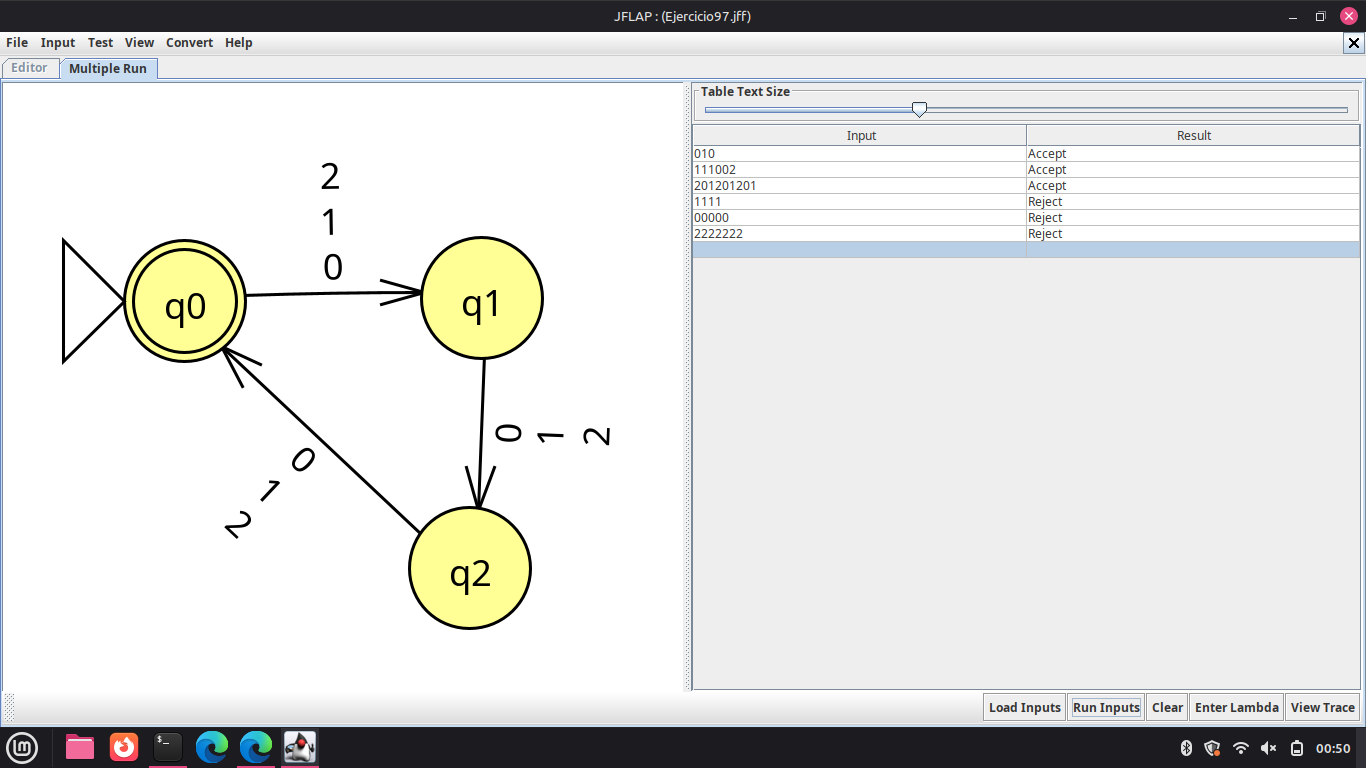
\includegraphics[width=0.95\textwidth]{evidencias/Ejercicio97.png}
    \caption{Diagrama y pruebas del AFD correspondiente al ejercicio 97 en JFLAP.}
\end{figure}
\begin{enunciado}{99}
Las palabras de $\Sigma_1$ que terminan con la cadena $001001$.
\end{enunciado}
\subsection*{Procedimiento}

Se requiere construir un AFD que acepte todas las cadenas sobre el alfabeto
\[
\Sigma_1=\{0,1,2\}
\]
que terminen exactamente con la secuencia
\[
001001.
\]

Para construir el autómata, cada estado representa el avance que se ha
realizado en el reconocimiento de la secuencia final $001001$.

\begin{itemize}
    \item $q_0$: todavía no se ha reconocido ningún símbolo de la secuencia.
    \item $q_1$: se ha reconocido $0$.
    \item $q_2$: se ha reconocido $00$.
    \item $q_3$: se ha reconocido $001$.
    \item $q_4$: se ha reconocido $0010$.
    \item $q_5$: se ha reconocido $00100$.
    \item $q_6$: se ha reconocido $001001$.
\end{itemize}

El estado inicial es $q_0$ y el único estado de aceptación es $q_6$.

Por lo tanto, el autómata se define formalmente como

\[
M=(Q,\Sigma,\delta,q_0,F)
\]

donde

\[
Q=\{q_0,q_1,q_2,q_3,q_4,q_5,q_6\},
\]

\[
\Sigma=\{0,1,2\},
\]

\[
F=\{q_6\}.
\]

\subsection*{Tabla de transición}

\begin{center}
\begin{tabular}{c|ccc}
Estado & 0 & 1 & 2 \\ \hline
$\rightarrow q_0$ & $q_1$ & $q_0$ & $q_0$ \\
$q_1$ & $q_2$ & $q_0$ & $q_0$ \\
$q_2$ & $q_2$ & $q_3$ & $q_0$ \\
$q_3$ & $q_4$ & $q_0$ & $q_0$ \\
$q_4$ & $q_5$ & $q_0$ & $q_0$ \\
$q_5$ & $q_2$ & $q_6$ & $q_0$ \\
$*q_6$ & $q_4$ & $q_0$ & $q_0$
\end{tabular}
\end{center}

Al llegar a $q_6$ se ha reconocido la secuencia completa $001001$.
Sin embargo, si aparecen más símbolos, el autómata debe continuar
procesándolos, ya que la condición establece que la cadena debe
\textbf{terminar} en $001001$.

Por ejemplo, desde $q_6$, al recibir un $0$ se pasa a $q_4$, debido a que
la cadena resultante conserva el sufijo $0010$, que también corresponde
al inicio de la secuencia buscada.

\subsection*{Pruebas}

Se realizaron las siguientes pruebas en JFLAP:

\begin{center}
\begin{tabular}{c|c}
Cadena & Resultado esperado \\ \hline
001001 & Aceptada \\
1001001 & Aceptada \\
212001001 & Aceptada \\
00100 & Rechazada \\
0010010 & Rechazada \\
0010012 & Rechazada
\end{tabular}
\end{center}

Las primeras tres cadenas terminan en $001001$, mientras que las últimas
tres no cumplen completamente con esta condición.

\subsection*{Evidencia en JFLAP}

\begin{figure}[H]
    \centering
    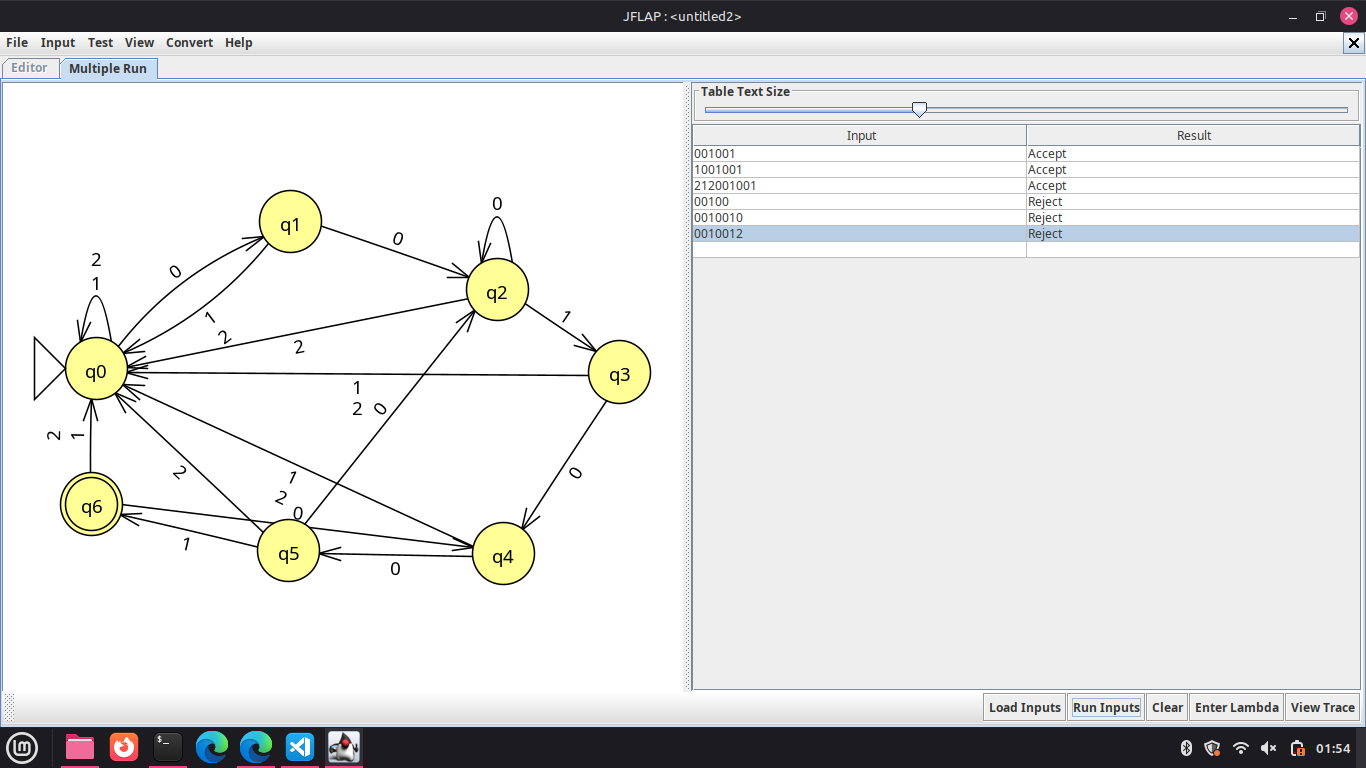
\includegraphics[width=0.95\textwidth]{evidencias/Ejercicio99.png}
    \caption{Diagrama y pruebas del AFD correspondiente al ejercicio 99 en JFLAP.}
\end{figure}

\begin{enunciado}{102}
Las palabras de $\Sigma_3$ que contienen la cadena $abbbab$.
\end{enunciado}
\subsection*{Procedimiento}

Se requiere construir un AFD sobre el alfabeto

\[
\Sigma_3=\{a,b\}
\]

que acepte todas las palabras que contengan la subcadena

\[
abbbab.
\]

Para construir el autómata, cada estado representa el avance realizado
en el reconocimiento de la subcadena $abbbab$.

\begin{itemize}
    \item $q_0$: todavía no se ha reconocido ningún símbolo de la subcadena.
    \item $q_1$: se ha reconocido $a$.
    \item $q_2$: se ha reconocido $ab$.
    \item $q_3$: se ha reconocido $abb$.
    \item $q_4$: se ha reconocido $abbb$.
    \item $q_5$: se ha reconocido $abbba$.
    \item $q_6$: se ha reconocido completamente $abbbab$.
\end{itemize}

El estado inicial es $q_0$ y el estado de aceptación es $q_6$.

Formalmente, el autómata se define como

\[
M=(Q,\Sigma,\delta,q_0,F)
\]

donde

\[
Q=\{q_0,q_1,q_2,q_3,q_4,q_5,q_6\},
\]

\[
\Sigma=\{a,b\},
\]

y

\[
F=\{q_6\}.
\]

\subsection*{Tabla de transición}

\begin{center}
\begin{tabular}{c|cc}
Estado & $a$ & $b$ \\ \hline
$\rightarrow q_0$ & $q_1$ & $q_0$ \\
$q_1$ & $q_1$ & $q_2$ \\
$q_2$ & $q_1$ & $q_3$ \\
$q_3$ & $q_1$ & $q_4$ \\
$q_4$ & $q_5$ & $q_0$ \\
$q_5$ & $q_1$ & $q_6$ \\
$*q_6$ & $q_6$ & $q_6$
\end{tabular}
\end{center}

Una vez que el autómata llega al estado $q_6$, la subcadena $abbbab$
ya fue encontrada. Por esta razón, cualquier símbolo posterior mantiene
al autómata en $q_6$, ya que la palabra continúa conteniendo la subcadena
solicitada.

\subsection*{Pruebas}

Se realizaron las siguientes pruebas en JFLAP:

\begin{center}
\begin{tabular}{c|c}
Cadena & Resultado esperado \\ \hline
abbbab & Aceptada \\
aabbbab & Aceptada \\
bbabbbaba & Aceptada \\
abbba & Rechazada \\
abbbba & Rechazada \\
ababab & Rechazada
\end{tabular}
\end{center}

Las primeras tres cadenas contienen la subcadena $abbbab$, mientras que
las últimas tres no la contienen completamente.

\subsection*{Evidencia en JFLAP}

\begin{figure}[H]
    \centering
    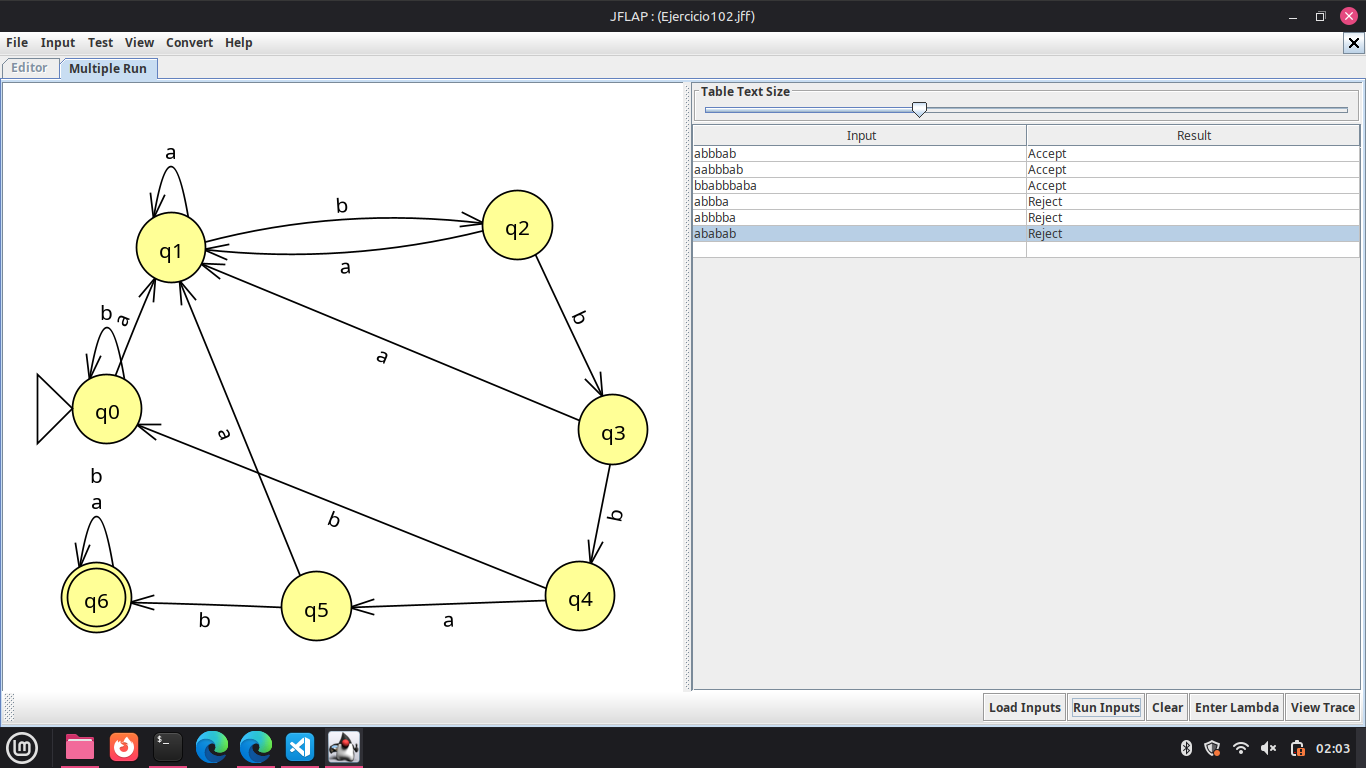
\includegraphics[width=0.95\textwidth]{evidencias/Ejercicio102.png}
    \caption{Diagrama y pruebas del AFD correspondiente al ejercicio 102 en JFLAP.}
\end{figure}

\begin{enunciado}{103}
Las palabras de $\Sigma_3$ que contienen la cadena $aabbba$.
\end{enunciado}
\subsection*{Procedimiento}

Se requiere construir un AFD sobre el alfabeto

\[
\Sigma_3=\{a,b\}
\]

que acepte todas las palabras que contengan la subcadena

\[
aabbba.
\]

Para construir el autómata, cada estado representa el avance realizado
en el reconocimiento de la subcadena $aabbba$.

\begin{itemize}
    \item $q_0$: todavía no se ha reconocido ningún símbolo de la subcadena.
    \item $q_1$: se ha reconocido $a$.
    \item $q_2$: se ha reconocido $aa$.
    \item $q_3$: se ha reconocido $aab$.
    \item $q_4$: se ha reconocido $aabb$.
    \item $q_5$: se ha reconocido $aabbb$.
    \item $q_6$: se ha reconocido completamente $aabbba$.
\end{itemize}

El estado inicial es $q_0$ y el estado de aceptación es $q_6$.

Formalmente, el autómata se define como

\[
M=(Q,\Sigma,\delta,q_0,F)
\]

donde

\[
Q=\{q_0,q_1,q_2,q_3,q_4,q_5,q_6\},
\]

\[
\Sigma=\{a,b\},
\]

y

\[
F=\{q_6\}.
\]

\subsection*{Tabla de transición}

\begin{center}
\begin{tabular}{c|cc}
Estado & $a$ & $b$ \\ \hline
$\rightarrow q_0$ & $q_1$ & $q_0$ \\
$q_1$ & $q_2$ & $q_0$ \\
$q_2$ & $q_2$ & $q_3$ \\
$q_3$ & $q_1$ & $q_4$ \\
$q_4$ & $q_1$ & $q_5$ \\
$q_5$ & $q_6$ & $q_0$ \\
$*q_6$ & $q_6$ & $q_6$
\end{tabular}
\end{center}

Una vez que el autómata alcanza el estado $q_6$, significa que la
subcadena $aabbba$ ya apareció dentro de la palabra. Por esta razón,
$q_6$ permanece como estado de aceptación sin importar si posteriormente
se recibe una $a$ o una $b$.

\subsection*{Pruebas}

Se realizaron las siguientes pruebas en JFLAP:

\begin{center}
\begin{tabular}{c|c}
Cadena & Resultado esperado \\ \hline
aabbba & Aceptada \\
baabbbab & Aceptada \\
aaaabbba & Aceptada \\
aabbb & Rechazada \\
aabbab & Rechazada \\
abbbab & Rechazada
\end{tabular}
\end{center}

Las primeras tres cadenas contienen la subcadena $aabbba$, mientras que
las últimas tres no contienen completamente la secuencia solicitada.

\subsection*{Evidencia en JFLAP}

\begin{figure}[H]
    \centering
    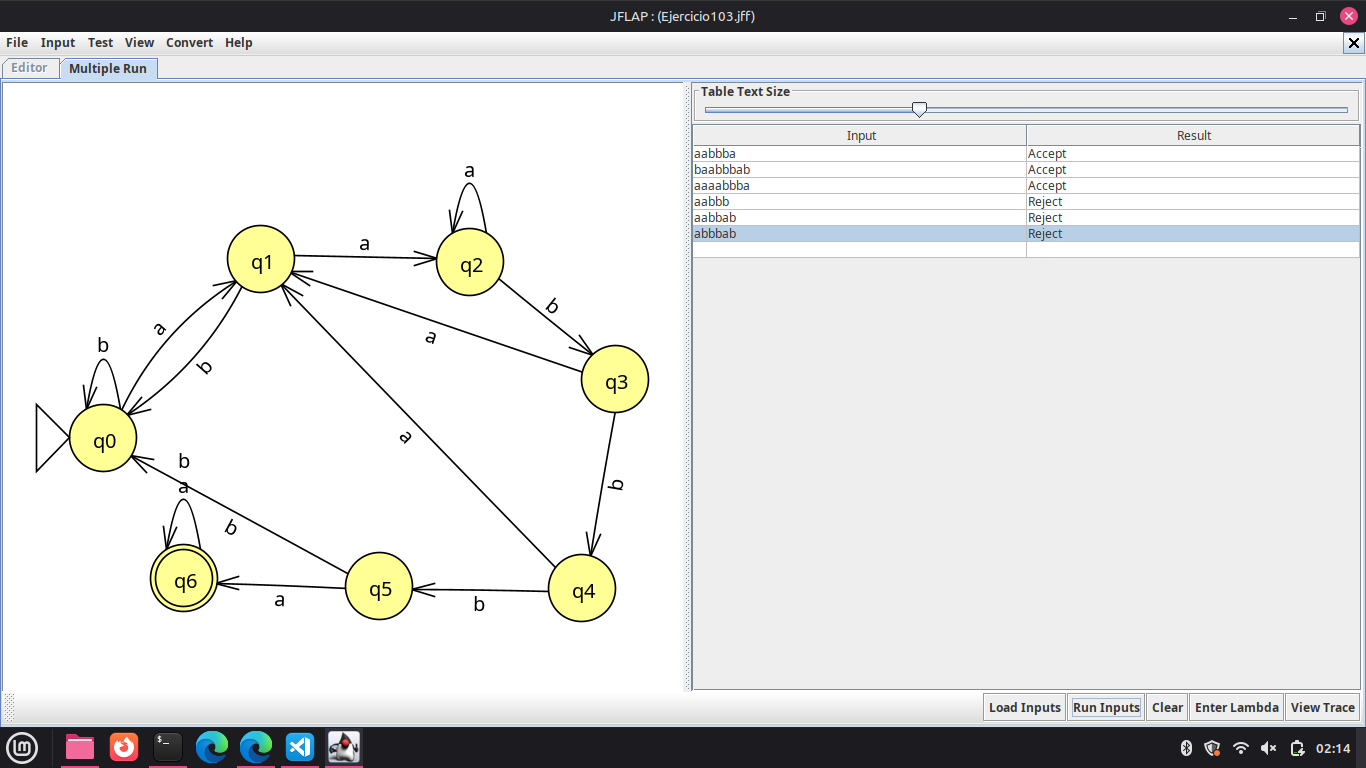
\includegraphics[width=0.95\textwidth]{evidencias/Ejercicio103.png}
    \caption{Diagrama y pruebas del AFD correspondiente al ejercicio 103 en JFLAP.}
\end{figure}

\begin{enunciado}{106}
Las palabras de $\Sigma_1$ que incluyen la subcadena $1101001$.
\end{enunciado}
\subsection*{Procedimiento}

Se requiere construir un AFD sobre el alfabeto

\[
\Sigma_1=\{0,1,2\}
\]

que acepte todas las palabras que incluyan la subcadena

\[
1101001.
\]

Para construir el autómata, cada estado representa el avance realizado
en el reconocimiento de la subcadena $1101001$.

\begin{itemize}
    \item $q_0$: todavía no se ha reconocido ningún símbolo.
    \item $q_1$: se ha reconocido $1$.
    \item $q_2$: se ha reconocido $11$.
    \item $q_3$: se ha reconocido $110$.
    \item $q_4$: se ha reconocido $1101$.
    \item $q_5$: se ha reconocido $11010$.
    \item $q_6$: se ha reconocido $110100$.
    \item $q_7$: se ha reconocido completamente $1101001$.
\end{itemize}

El estado inicial es $q_0$ y el estado de aceptación es $q_7$.

Formalmente,

\[
M=(Q,\Sigma,\delta,q_0,F)
\]

donde

\[
Q=\{q_0,q_1,q_2,q_3,q_4,q_5,q_6,q_7\},
\]

\[
\Sigma=\{0,1,2\},
\]

y

\[
F=\{q_7\}.
\]

\subsection*{Tabla de transición}

\begin{center}
\begin{tabular}{c|ccc}
Estado & $0$ & $1$ & $2$ \\ \hline
$\rightarrow q_0$ & $q_0$ & $q_1$ & $q_0$ \\
$q_1$ & $q_0$ & $q_2$ & $q_0$ \\
$q_2$ & $q_3$ & $q_2$ & $q_0$ \\
$q_3$ & $q_0$ & $q_4$ & $q_0$ \\
$q_4$ & $q_5$ & $q_2$ & $q_0$ \\
$q_5$ & $q_6$ & $q_1$ & $q_0$ \\
$q_6$ & $q_0$ & $q_7$ & $q_0$ \\
$*q_7$ & $q_7$ & $q_7$ & $q_7$
\end{tabular}
\end{center}

Cuando el autómata alcanza $q_7$, significa que la subcadena
$1101001$ ya apareció dentro de la palabra. Por esta razón, cualquier
símbolo posterior mantiene al autómata en $q_7$.

\subsection*{Pruebas}

Se realizaron las siguientes pruebas en JFLAP:

\begin{center}
\begin{tabular}{c|c}
Cadena & Resultado esperado \\ \hline
1101001 & Aceptada \\
01101001 & Aceptada \\
211010012 & Aceptada \\
110100 & Rechazada \\
110101 & Rechazada \\
1101002 & Rechazada
\end{tabular}
\end{center}

Las primeras tres cadenas incluyen la subcadena $1101001$, mientras que
las últimas tres no contienen completamente la secuencia solicitada.

\subsection*{Evidencia en JFLAP}

\begin{figure}[H]
    \centering
    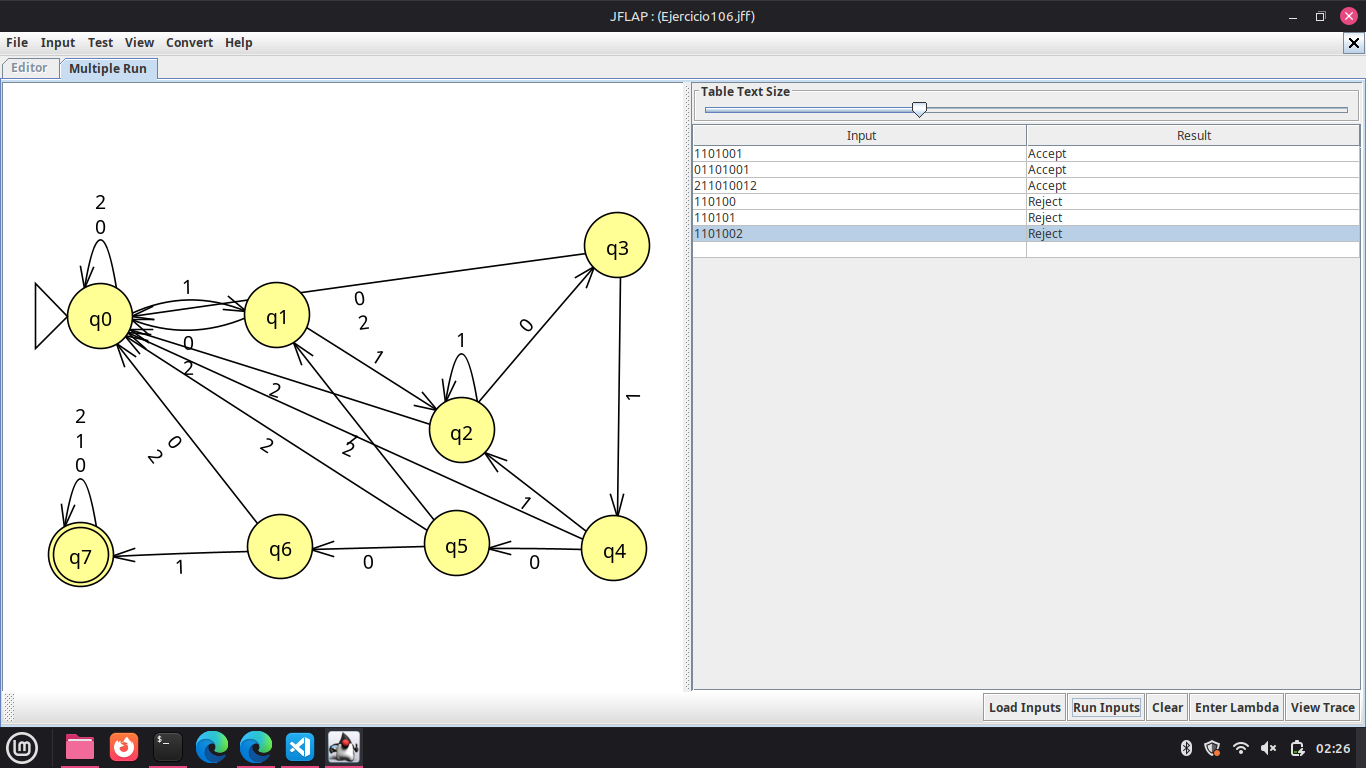
\includegraphics[width=0.95\textwidth]{evidencias/Ejercicio106.png}
    \caption{Diagrama y pruebas del AFD correspondiente al ejercicio 106 en JFLAP.}
\end{figure}

\begin{enunciado}{107}
Las palabras de $\Sigma_1$ que incluyen al menos una vez la subcadena
$0101$ y al menos una vez la subcadena $021$.
\end{enunciado}
\subsection*{Procedimiento}

Se requiere construir un AFD sobre el alfabeto

\[
\Sigma_1=\{0,1,2\}
\]

que acepte todas las palabras que incluyan al menos una vez la subcadena
$0101$ y al menos una vez la subcadena $021$.

Para construir el autómata se consideran tres situaciones principales:
primero, cuando todavía no se ha encontrado ninguna de las dos
subcadenas; segundo, cuando ya se encontró $0101$ y se continúa buscando
$021$; y tercero, cuando ya se encontró $021$ y se continúa buscando
$0101$.

Cuando ambas subcadenas han sido encontradas, el autómata alcanza el
estado de aceptación $q_{12}$.

Formalmente,

\[
M=(Q,\Sigma,\delta,q_0,F)
\]

donde

\[
Q=\{q_0,q_1,q_2,q_3,q_4,q_5,q_6,q_7,
q_8,q_9,q_{10},q_{11},q_{12}\},
\]

\[
\Sigma=\{0,1,2\},
\]

y

\[
F=\{q_{12}\}.
\]

\subsection*{Tabla de transición}

\begin{center}
\begin{tabular}{c|ccc}
Estado & $0$ & $1$ & $2$ \\ \hline
$\rightarrow q_0$ & $q_1$ & $q_0$ & $q_0$ \\
$q_1$ & $q_1$ & $q_2$ & $q_4$ \\
$q_2$ & $q_3$ & $q_0$ & $q_0$ \\
$q_3$ & $q_1$ & $q_5$ & $q_4$ \\
$q_4$ & $q_1$ & $q_8$ & $q_0$ \\
$q_5$ & $q_6$ & $q_5$ & $q_5$ \\
$q_6$ & $q_6$ & $q_5$ & $q_7$ \\
$q_7$ & $q_6$ & $q_{12}$ & $q_5$ \\
$q_8$ & $q_9$ & $q_8$ & $q_8$ \\
$q_9$ & $q_9$ & $q_{10}$ & $q_8$ \\
$q_{10}$ & $q_{11}$ & $q_8$ & $q_8$ \\
$q_{11}$ & $q_9$ & $q_{12}$ & $q_8$ \\
$*q_{12}$ & $q_{12}$ & $q_{12}$ & $q_{12}$
\end{tabular}
\end{center}

Los estados $q_5$, $q_6$ y $q_7$ representan situaciones en las que
la subcadena $0101$ ya fue encontrada y todavía se busca $021$.

Los estados $q_8$, $q_9$, $q_{10}$ y $q_{11}$ representan situaciones
en las que $021$ ya fue encontrada y todavía se busca $0101$.

Finalmente, al llegar a $q_{12}$ significa que ambas subcadenas ya
aparecieron. Por esta razón, las entradas $0$, $1$ y $2$ mantienen al
autómata en este estado de aceptación.

\subsection*{Pruebas}

Se realizaron las siguientes pruebas en JFLAP:

\begin{center}
\begin{tabular}{c|c}
Cadena & Resultado esperado \\ \hline
0101021 & Aceptada \\
0210101 & Aceptada \\
201010210 & Aceptada \\
0101 & Rechazada \\
021 & Rechazada \\
010201 & Rechazada
\end{tabular}
\end{center}

Las primeras tres cadenas contienen tanto la subcadena $0101$ como
la subcadena $021$. Las últimas tres no cumplen simultáneamente ambas
condiciones.

\subsection*{Evidencia en JFLAP}

\begin{figure}[H]
    \centering
    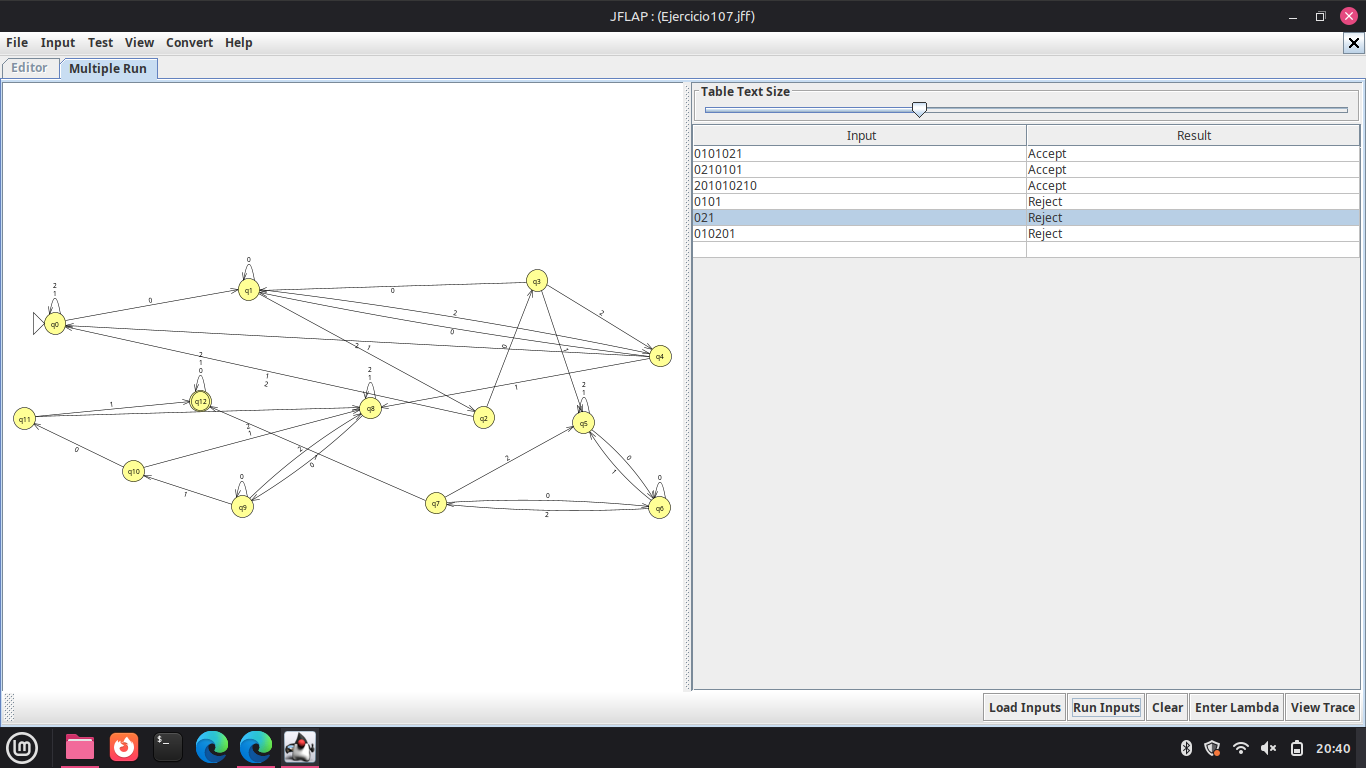
\includegraphics[width=0.95\textwidth]{evidencias/Ejercicio107.png}
    \caption{Diagrama y pruebas del AFD correspondiente al ejercicio 107 en JFLAP.}
\end{figure}

\begin{enunciado}{109}
Las palabras de $\Sigma_2$ que incluyen al menos una vez la subcadena
$abbcb$ y al menos una vez la subcadena $cbaabb$, asumiendo que sí se pueden
traslapar.
\end{enunciado}


\begin{enunciado}{111}
Las palabras de $\Sigma_1$ que contienen exactamente tres veces la
subcadena $01002$.
\end{enunciado}
\subsection*{Procedimiento}

Se requiere construir un AFD sobre el alfabeto

\[
\Sigma_1=\{0,1,2\}
\]

que acepte únicamente las palabras que contengan exactamente tres veces
la subcadena $01002$.

Para construir el autómata se lleva un registro tanto del número de veces
que se ha encontrado la subcadena como del avance que se tiene en una
posible nueva aparición de $01002$.

Los estados se dividen en cuatro grupos principales:

\begin{itemize}
    \item $q_0$ a $q_4$: todavía no se ha encontrado $01002$.
    \item $q_5$ a $q_9$: se ha encontrado exactamente una vez.
    \item $q_{10}$ a $q_{14}$: se ha encontrado exactamente dos veces.
    \item $q_{15}$ a $q_{19}$: se ha encontrado exactamente tres veces.
\end{itemize}

Finalmente, $q_{20}$ es un estado trampa al que se llega cuando la
subcadena aparece por cuarta vez.

Formalmente,

\[
M=(Q,\Sigma,\delta,q_0,F)
\]

donde

\[
Q=\{q_0,q_1,q_2,\ldots,q_{20}\},
\]

\[
\Sigma=\{0,1,2\},
\]

y el conjunto de estados finales es

\[
F=\{q_{15},q_{16},q_{17},q_{18},q_{19}\}.
\]

\subsection*{Tabla de transición}

\begin{center}
\begin{tabular}{c|ccc}
Estado & $0$ & $1$ & $2$ \\ \hline

$\rightarrow q_0$ & $q_1$ & $q_0$ & $q_0$ \\
$q_1$ & $q_1$ & $q_2$ & $q_0$ \\
$q_2$ & $q_3$ & $q_0$ & $q_0$ \\
$q_3$ & $q_4$ & $q_2$ & $q_0$ \\
$q_4$ & $q_1$ & $q_2$ & $q_5$ \\ \hline

$q_5$ & $q_6$ & $q_5$ & $q_5$ \\
$q_6$ & $q_6$ & $q_7$ & $q_5$ \\
$q_7$ & $q_8$ & $q_5$ & $q_5$ \\
$q_8$ & $q_9$ & $q_7$ & $q_5$ \\
$q_9$ & $q_6$ & $q_7$ & $q_{10}$ \\ \hline

$q_{10}$ & $q_{11}$ & $q_{10}$ & $q_{10}$ \\
$q_{11}$ & $q_{11}$ & $q_{12}$ & $q_{10}$ \\
$q_{12}$ & $q_{13}$ & $q_{10}$ & $q_{10}$ \\
$q_{13}$ & $q_{14}$ & $q_{12}$ & $q_{10}$ \\
$q_{14}$ & $q_{11}$ & $q_{12}$ & $q_{15}$ \\ \hline

$*q_{15}$ & $q_{16}$ & $q_{15}$ & $q_{15}$ \\
$*q_{16}$ & $q_{16}$ & $q_{17}$ & $q_{15}$ \\
$*q_{17}$ & $q_{18}$ & $q_{15}$ & $q_{15}$ \\
$*q_{18}$ & $q_{19}$ & $q_{17}$ & $q_{15}$ \\
$*q_{19}$ & $q_{16}$ & $q_{17}$ & $q_{20}$ \\ \hline

$q_{20}$ & $q_{20}$ & $q_{20}$ & $q_{20}$

\end{tabular}
\end{center}

Los estados $q_{15}$ a $q_{19}$ son estados de aceptación debido a que
representan situaciones en las que la subcadena $01002$ ya apareció
exactamente tres veces.

Aunque se haya encontrado tres veces, el autómata continúa verificando
la entrada. Si se completa una cuarta aparición de $01002$, se llega
al estado $q_{20}$.

El estado $q_{20}$ es un estado trampa, ya que una palabra que contiene
cuatro o más apariciones de $01002$ ya no puede cumplir la condición de
contenerla exactamente tres veces.

\subsection*{Pruebas}

Se realizaron las siguientes pruebas en JFLAP:

\begin{center}
\begin{tabular}{c|c}
Cadena & Resultado esperado \\ \hline
010020100201002 & Aceptada \\
10100201002010022 & Aceptada \\
010020100201002111 & Aceptada \\
0100201002 & Rechazada \\
01002 & Rechazada \\
01002010020100201002 & Rechazada
\end{tabular}
\end{center}

Las primeras tres cadenas contienen exactamente tres apariciones de
$01002$. Las siguientes contienen una cantidad diferente de tres y,
por lo tanto, son rechazadas.

\subsection*{Evidencia en JFLAP}

\begin{figure}[H]
    \centering
    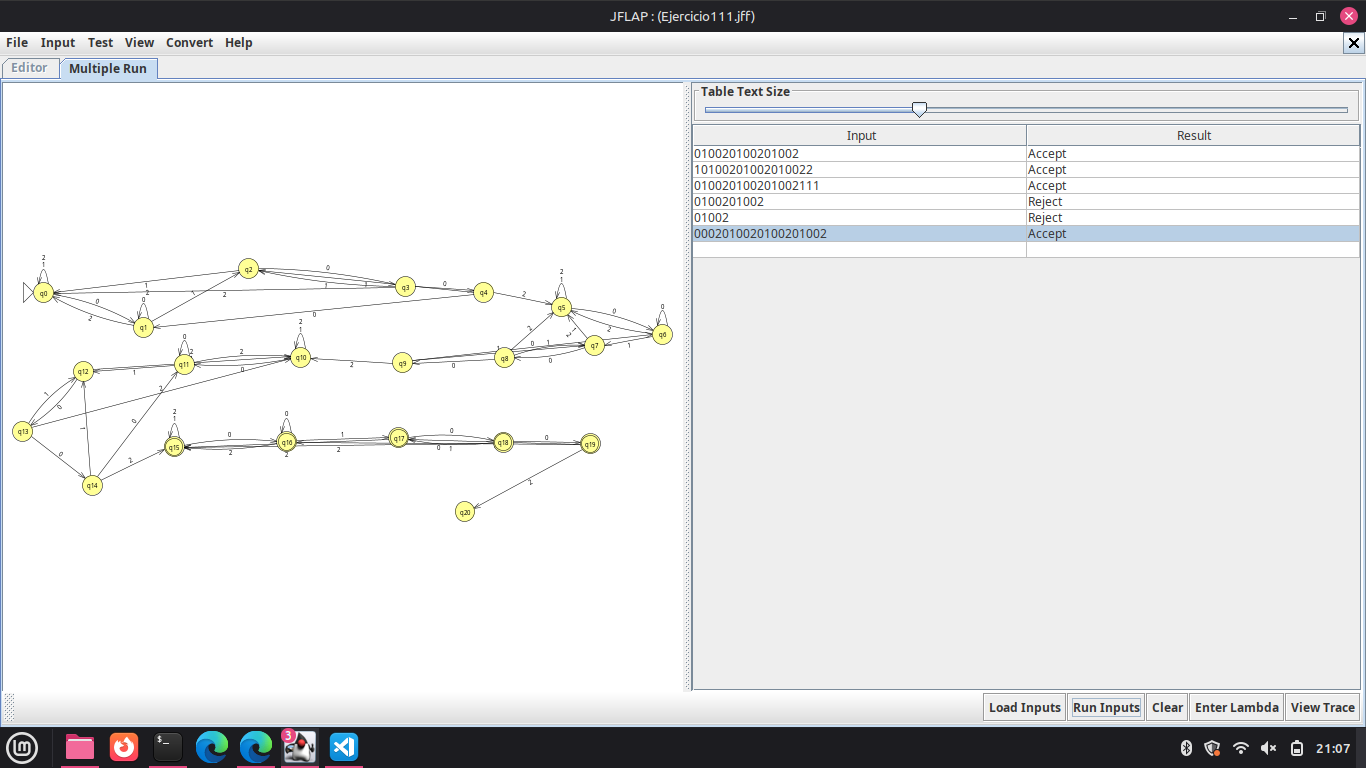
\includegraphics[width=0.95\textwidth]{evidencias/Ejercicio111.png}
    \caption{Diagrama y pruebas del AFD correspondiente al ejercicio 111 en JFLAP.}
\end{figure}

\begin{enunciado}{112}
Las palabras de $\Sigma_1$ que contienen dos veces la subcadena $010$,
asumiendo que no se pueden traslapar; es decir, que $01010$ no está en el
lenguaje, mientras que $010010$ sí pertenece.
\end{enunciado}
\subsection*{Procedimiento}

Se construyó un AFD sobre $\Sigma_1=\{0,1,2\}$ que reconoce las palabras
que contienen dos veces la subcadena $010$, sin permitir traslapes.

Cuando se encuentra la primera aparición de $010$, el último símbolo de
esta aparición no se reutiliza como inicio de la siguiente. De esta manera,
por ejemplo, $01010$ no es aceptada, mientras que $010010$ sí lo es.

El estado inicial es $q_0$ y el estado de aceptación es $q_6$.

\subsection*{Tabla de transición}

\begin{center}
\begin{tabular}{c|ccc}
Estado & 0 & 1 & 2 \\ \hline
$\rightarrow q_0$ & $q_1$ & $q_0$ & $q_0$ \\
$q_1$ & $q_1$ & $q_2$ & $q_0$ \\
$q_2$ & $q_3$ & $q_0$ & $q_0$ \\
$q_3$ & $q_4$ & $q_3$ & $q_3$ \\
$q_4$ & $q_4$ & $q_5$ & $q_3$ \\
$q_5$ & $q_6$ & $q_3$ & $q_3$ \\
$*q_6$ & $q_6$ & $q_6$ & $q_6$
\end{tabular}
\end{center}

\subsection*{Pruebas}

\begin{center}
\begin{tabular}{c|c}
Cadena & Resultado \\ \hline
010010 & Aceptada \\
0101010 & Aceptada \\
20100102 & Aceptada \\
01010 & Rechazada \\
010 & Rechazada \\
001010 & Rechazada
\end{tabular}
\end{center}

\subsection*{Evidencia en JFLAP}

\begin{figure}[H]
\centering
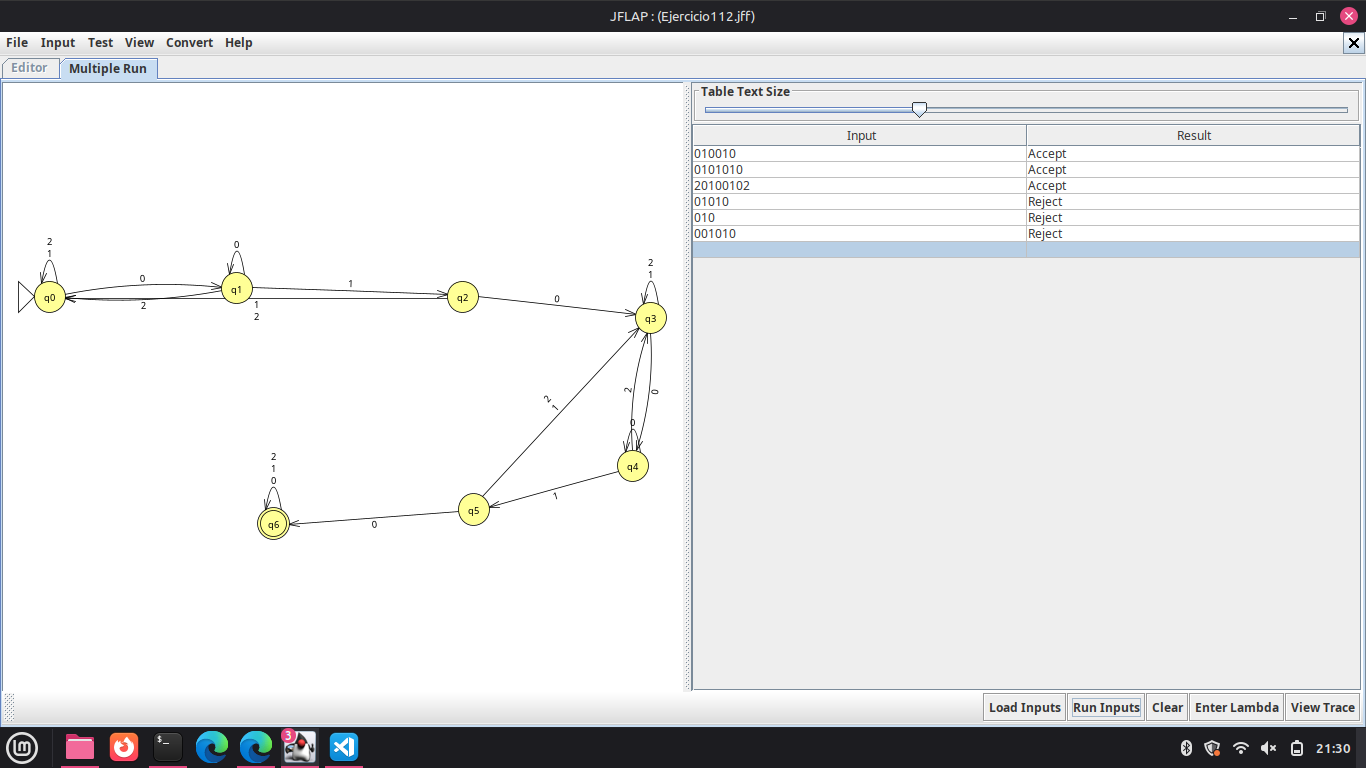
\includegraphics[width=0.95\textwidth]{evidencias/Ejercicio112.png}
\caption{AFD y pruebas correspondientes al ejercicio 112.}
\end{figure}

\begin{enunciado}{113}
Las palabras de $\Sigma_1$ que contienen dos veces la subcadena $010$,
asumiendo que sí se pueden traslapar.
\end{enunciado}
\subsection*{Procedimiento}

Se construyó un AFD sobre $\Sigma_1=\{0,1,2\}$ que reconoce las palabras
que contienen dos apariciones de la subcadena $010$, permitiendo
traslapes.

A diferencia del ejercicio anterior, al encontrar $010$, su último $0$
puede utilizarse también como el primer símbolo de una nueva aparición.
Por esta razón, la palabra $01010$ contiene dos apariciones traslapadas.

\subsection*{Tabla de transición}

\begin{center}
\begin{tabular}{c|ccc}
Estado & 0 & 1 & 2 \\ \hline
$\rightarrow q_0$ & $q_1$ & $q_0$ & $q_0$ \\
$q_1$ & $q_1$ & $q_2$ & $q_0$ \\
$q_2$ & $q_3$ & $q_0$ & $q_0$ \\
$q_3$ & $q_3$ & $q_4$ & $q_0$ \\
$q_4$ & $q_5$ & $q_0$ & $q_0$ \\
$*q_5$ & $q_5$ & $q_5$ & $q_5$
\end{tabular}
\end{center}

\subsection*{Pruebas}

\begin{center}
\begin{tabular}{c|c}
Cadena & Resultado \\ \hline
01010 & Aceptada \\
010010 & Aceptada \\
2010102 & Aceptada \\
010 & Rechazada \\
0010 & Rechazada \\
01012 & Rechazada
\end{tabular}
\end{center}

\begin{figure}[H]
\centering
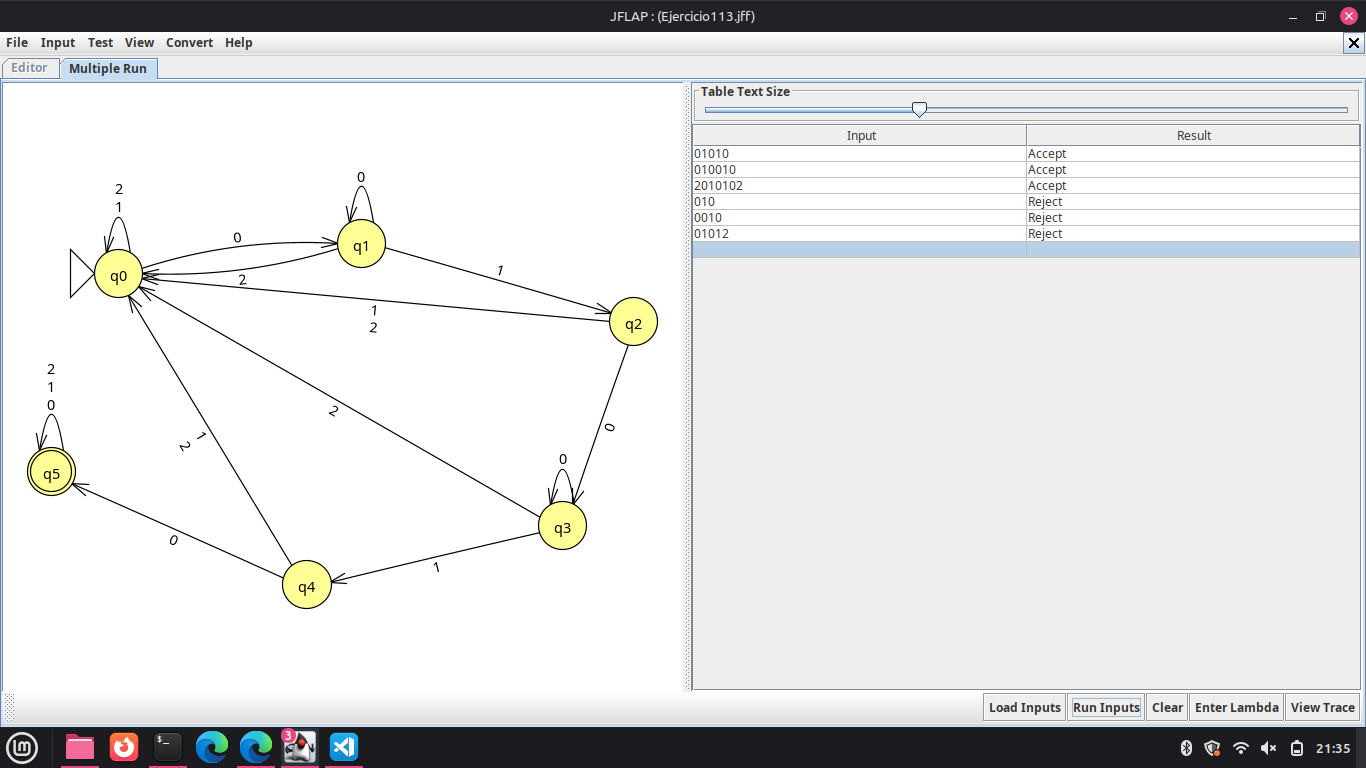
\includegraphics[width=0.95\textwidth]{evidencias/Ejercicio113.png}
\caption{AFD y pruebas correspondientes al ejercicio 113.}
\end{figure}

\begin{enunciado}{116}
\[
L=\{w\in\Sigma_2 : w=a^n b^m c^{n+1},\; m,n\in\mathbb{N}\}.
\]
\end{enunciado}


\begin{enunciado}{118}
\[
L=\{w\in\Sigma_3 : w=axabya,\; x,y\in\Sigma_3^*\}.
\]
\end{enunciado}
\subsection*{Procedimiento}

El lenguaje es

\[
L=\{w\in\Sigma_3^*:w=axabya,\ x,y\in\Sigma_3^*\}.
\]

El AFD verifica que la palabra comience con $a$, que posteriormente
aparezca la subcadena $ab$ y que finalmente termine en $a$.

El estado $q_5$ funciona como estado trampa para las palabras que
comienzan con $b$.

\subsection*{Tabla de transición}

\begin{center}
\begin{tabular}{c|cc}
Estado & a & b \\ \hline
$\rightarrow q_0$ & $q_1$ & $q_5$ \\
$q_1$ & $q_2$ & $q_1$ \\
$q_2$ & $q_2$ & $q_3$ \\
$q_3$ & $q_4$ & $q_3$ \\
$*q_4$ & $q_4$ & $q_3$ \\
$q_5$ & $q_5$ & $q_5$
\end{tabular}
\end{center}

\begin{figure}[H]
\centering
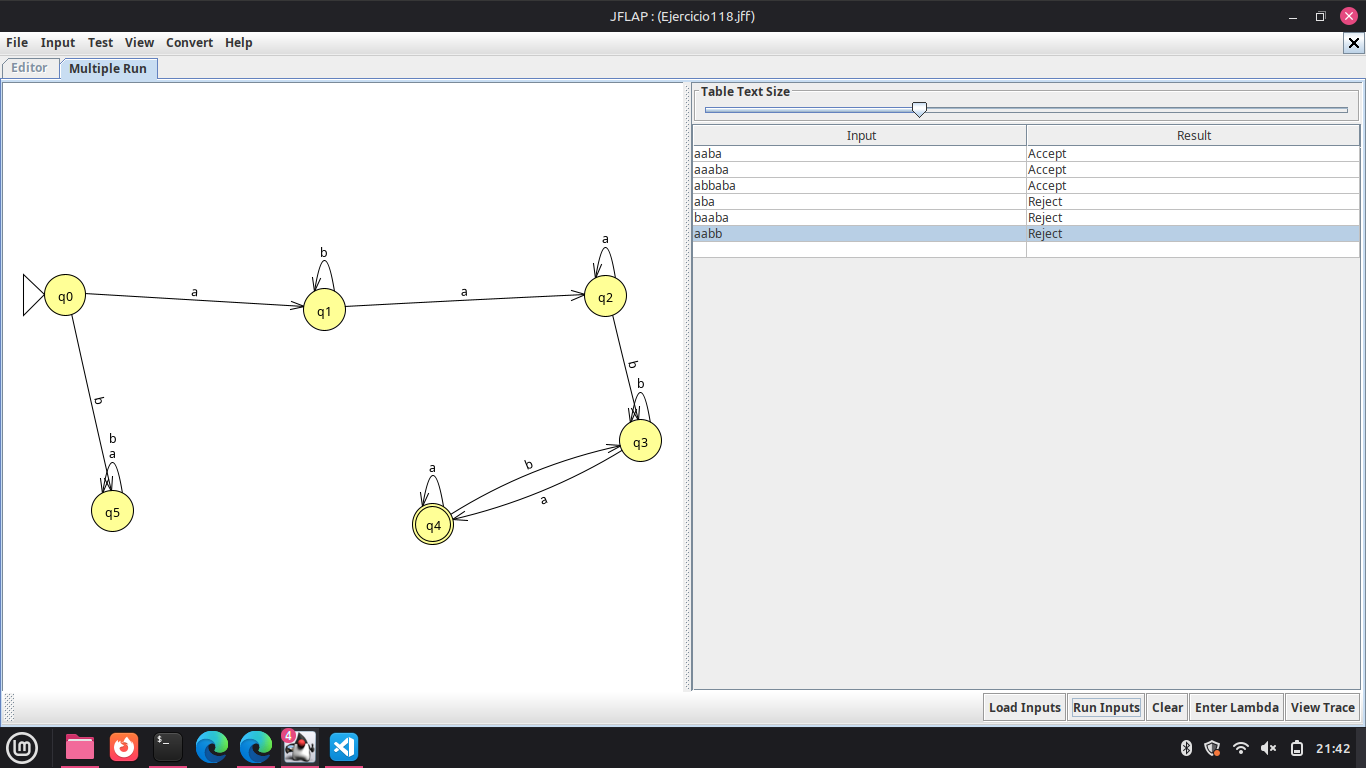
\includegraphics[width=0.95\textwidth]{evidencias/Ejercicio118.png}
\caption{AFD correspondiente al ejercicio 118.}
\end{figure}

\begin{enunciado}{120}
Las palabras de $\Sigma_1$ tales que el primer carácter y el último son
distintos.
\end{enunciado}
\subsection*{Procedimiento}

Se diseñó un AFD que recuerda el primer símbolo de la palabra y compara
dicho símbolo con el último carácter leído. Una palabra es aceptada
únicamente cuando ambos son diferentes.

\subsection*{Tabla de transición}

\begin{center}
\begin{tabular}{c|ccc}
Estado & 0 & 1 & 2 \\ \hline
$\rightarrow q_0$ & $q_1$ & $q_2$ & $q_3$ \\
$q_1$ & $q_1$ & $q_4$ & $q_4$ \\
$q_2$ & $q_5$ & $q_2$ & $q_5$ \\
$q_3$ & $q_6$ & $q_6$ & $q_3$ \\
$*q_4$ & $q_1$ & $q_4$ & $q_4$ \\
$*q_5$ & $q_5$ & $q_2$ & $q_5$ \\
$*q_6$ & $q_6$ & $q_6$ & $q_3$
\end{tabular}
\end{center}

\begin{figure}[H]
\centering
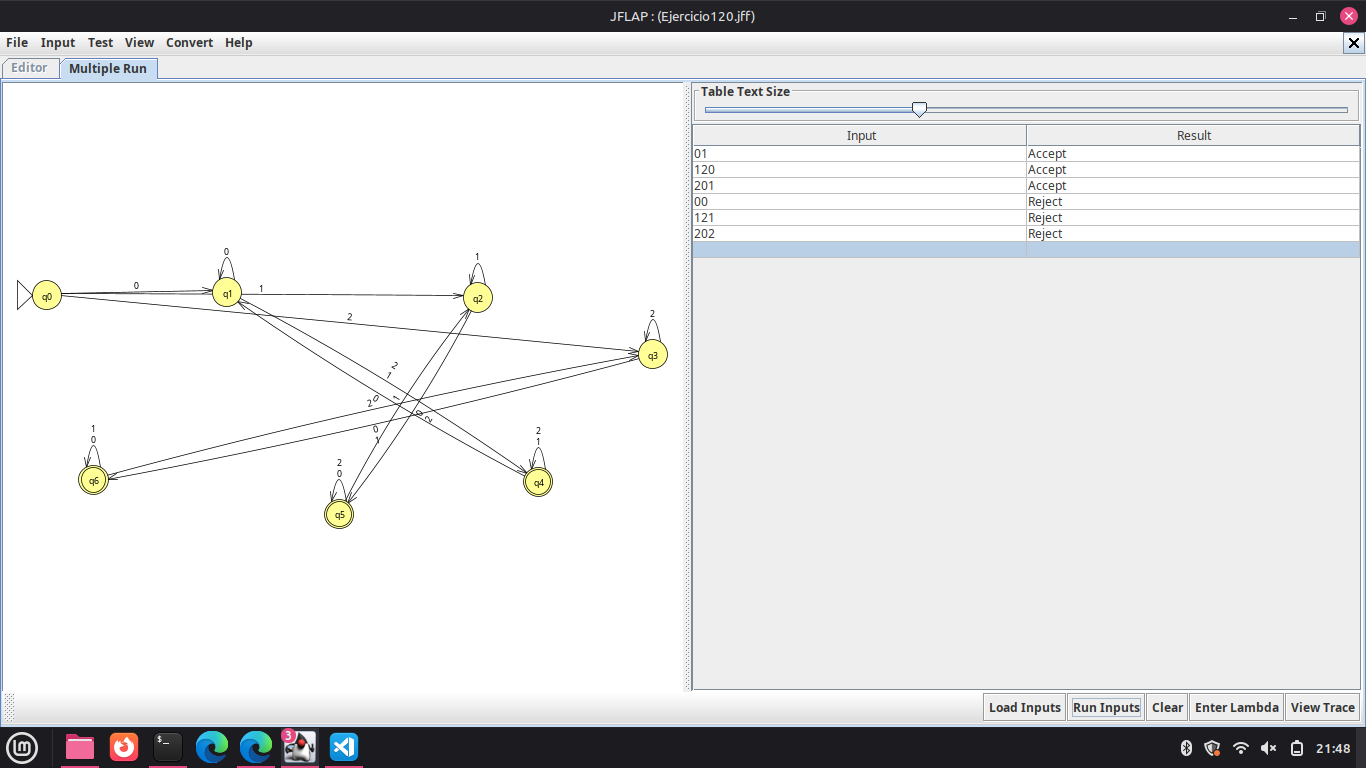
\includegraphics[width=0.95\textwidth]{evidencias/Ejercicio120.png}
\caption{AFD correspondiente al ejercicio 120.}
\end{figure}

\begin{enunciado}{121}
Las palabras de $\Sigma_1$ con longitud $3n$ para algún $n\in\mathbb{N}$,
tales que si se dividen en $n$ bloques de longitud 3, cada uno de éstos
tiene al menos un $0$.

Por ejemplo, $000\;011\;110\;101$ es una palabra válida, mientras que
$001\;101\;111\;010$ no lo es, pues el tercer bloque no tiene ningún $0$.
\end{enunciado}
\subsection*{Procedimiento}

La palabra se divide en bloques consecutivos de longitud 3. El AFD
verifica que cada bloque contenga al menos un símbolo $0$.

El estado $q_0$ representa que se terminó correctamente un bloque, por
lo que también es estado de aceptación. El estado $q_5$ es un estado
trampa al que se llega cuando se completa un bloque sin ningún $0$.

\subsection*{Tabla de transición}

\begin{center}
\begin{tabular}{c|ccc}
Estado & 0 & 1 & 2 \\ \hline
$\rightarrow *q_0$ & $q_1$ & $q_2$ & $q_2$ \\
$q_1$ & $q_3$ & $q_3$ & $q_3$ \\
$q_2$ & $q_3$ & $q_4$ & $q_4$ \\
$q_3$ & $q_0$ & $q_0$ & $q_0$ \\
$q_4$ & $q_0$ & $q_5$ & $q_5$ \\
$q_5$ & $q_5$ & $q_5$ & $q_5$
\end{tabular}
\end{center}

\begin{figure}[H]
\centering
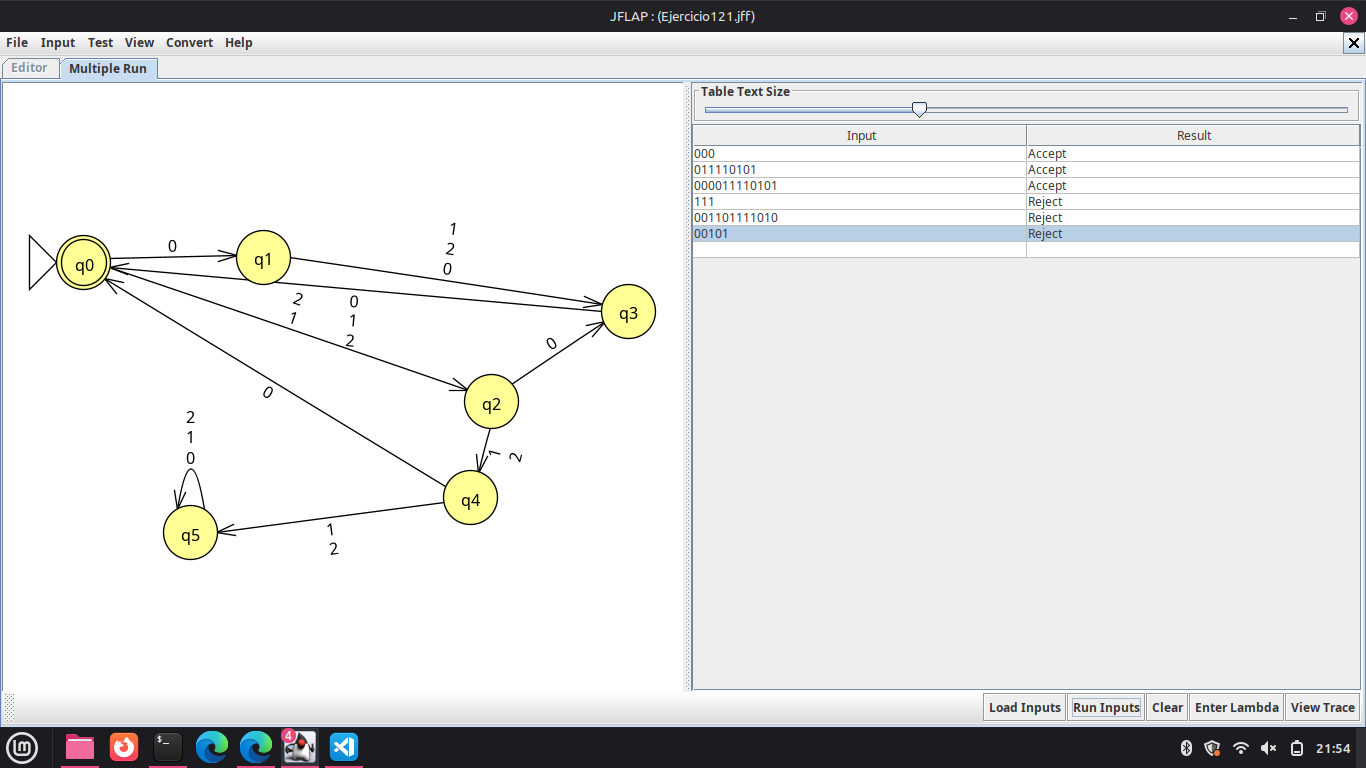
\includegraphics[width=0.95\textwidth]{evidencias/Ejercicio121.png}
\caption{AFD correspondiente al ejercicio 121.}
\end{figure}

\begin{enunciado}{122}
Las palabras de $\Sigma_1$ tales que cualquier cadena de tres símbolos
consecutivos debe tener un $0$.

Nota que la cadena $001110$ sí está en el lenguaje del problema anterior,
pero no en este, mientras que $00101$ está en el lenguaje de este problema
y no en el del anterior.
\end{enunciado}
\subsection*{Procedimiento}

El AFD verifica que cualquier conjunto de tres símbolos consecutivos
contenga al menos un $0$. Por lo tanto, nunca pueden aparecer tres
símbolos consecutivos pertenecientes solamente a $\{1,2\}$.

Los estados $q_0$, $q_1$ y $q_2$ son de aceptación. El estado $q_3$
es un estado trampa.

\subsection*{Tabla de transición}

\begin{center}
\begin{tabular}{c|ccc}
Estado & 0 & 1 & 2 \\ \hline
$\rightarrow *q_0$ & $q_0$ & $q_1$ & $q_1$ \\
$*q_1$ & $q_0$ & $q_2$ & $q_2$ \\
$*q_2$ & $q_0$ & $q_3$ & $q_3$ \\
$q_3$ & $q_3$ & $q_3$ & $q_3$
\end{tabular}
\end{center}

\begin{figure}[H]
\centering
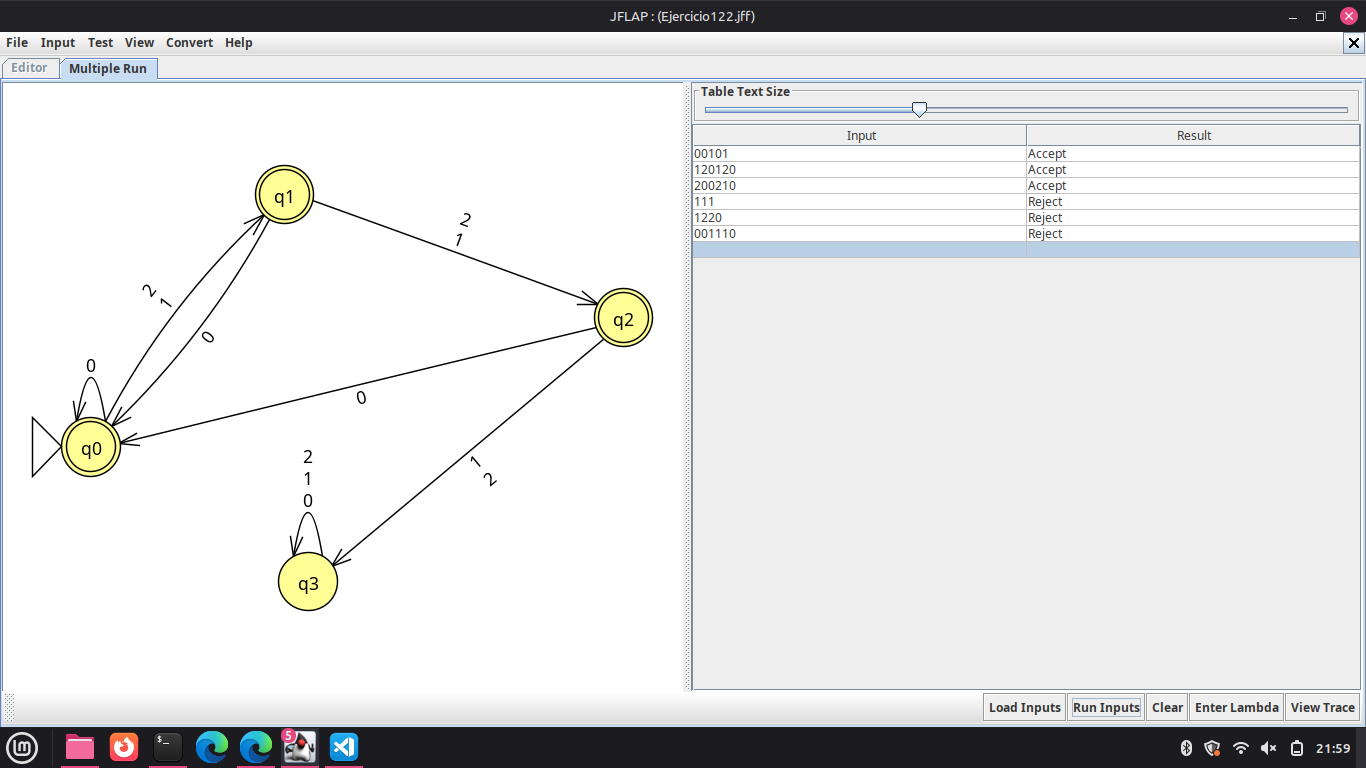
\includegraphics[width=0.95\textwidth]{evidencias/Ejercicio122.png}
\caption{AFD correspondiente al ejercicio 122.}
\end{figure}

\begin{enunciado}{123}
Las palabras de $\Sigma_3$ de la forma
\[
wxw
\]
donde $w\in\Sigma_3^2$ y $x\in\Sigma_3^*$.
\end{enunciado}


\begin{enunciado}{124}
En el siguiente diagrama, se muestra un mecanismo con palancas. Se suelta
una cadena de canicas ordenadas en las entradas $0$ y $1$, formando una
palabra del alfabeto $\Sigma=\{0,1\}$.

De esta forma, la palabra $0010$ significa que dos canicas caen por el
conducto $0$, luego se suelta una en $1$, terminando con una cuarta en $0$.

En el juego se encuentran tres palancas. Cada vez que una canica pasa por
una palanca, esta cambia de posición. Una palabra será aceptada si la
última canica sale por $A$ y será rechazada si la última canica sale por
$R$.

\begin{enumerate}[label=\alph*)]
    \item ¿De cuántas formas pueden estar colocadas las tres palancas?
    
    \item Realice un dibujo de cada uno de los estados en los que pueden
    estar colocadas e identifique cuál es el resultado de soltar una canica
    en $0$ o en $1$ en cada uno de los estados, así como la posición en la
    que quedarán las palancas después de cada caso.
    
    \item Encuentre la tabla de transiciones de un autómata finito
    determinista que describa si una palabra es aceptada o rechazada.
\end{enumerate}
\end{enunciado}


\begin{enunciado}{125}
Sea
\[
A=(Q,\Sigma,\delta,A_0,F)
\]
un autómata finito determinista.

¿Cuál es el lenguaje del autómata
\[
A=(Q,\Sigma,\delta,A_0,Q\setminus F)?
\]

Recuerde que
\[
A\setminus B=\{x:x\in A\text{ y }x\notin B\}.
\]
\end{enunciado}


\subsection*{Procedimiento}

Al sustituir el conjunto de estados finales $F$ por su complemento
$Q\setminus F$, las palabras que anteriormente eran aceptadas pasan a
ser rechazadas y las rechazadas pasan a ser aceptadas.

Por lo tanto, el lenguaje reconocido es el complemento del lenguaje
original:

\[
\boxed{L(A')=\Sigma^*\setminus L(A)}
\]


\begin{enunciado}{126}
Sea
\[
A=(Q,\Sigma,\delta,A_0,F)
\]
un autómata finito determinista.

¿Cuál es el lenguaje del autómata si
\[
F=\varnothing?
\]
\end{enunciado}
\subsection*{Procedimiento}

Si $F=\varnothing$, el autómata no posee ningún estado de aceptación.
Por lo tanto, ninguna palabra puede ser aceptada.

\[
\boxed{L(A)=\varnothing}
\]

\begin{enunciado}{127}
Sea
\[
A=(Q,\Sigma,\delta,q_0,F)
\]
un autómata finito determinista.

¿Cuál es el lenguaje del autómata si
\[
F=Q?
\]
\end{enunciado}
\subsection*{Procedimiento}

Si $F=Q$, todos los estados del autómata son estados de aceptación.
Por lo tanto, cualquier palabra sobre el alfabeto $\Sigma$ termina en
un estado final.

\[
\boxed{L(A)=\Sigma^*}
\]

\begin{enunciado}{128}
Sea $L$ el lenguaje del autómata dado por el siguiente diagrama.

Encuentre un autómata finito determinista que identifique el lenguaje
$L_2$ cuyas palabras son las palabras de $L$ quitándoles el último símbolo.

Es decir, si
\[
001001\in L,
\]
entonces
\[
00100\in L_2.
\]
\end{enunciado}
\subsection*{Procedimiento}

El lenguaje $L_2$ está formado por las palabras del lenguaje original
después de eliminar su último símbolo.

Para construir el nuevo autómata se conservan los estados y las
transiciones del AFD original. Posteriormente se identifican los estados
desde los cuales una transición adicional puede completar una palabra
aceptada por el autómata original.

De esta manera se obtiene el AFD correspondiente a $L_2$.

\subsection*{Evidencia en JFLAP}

\begin{figure}[H]
\centering
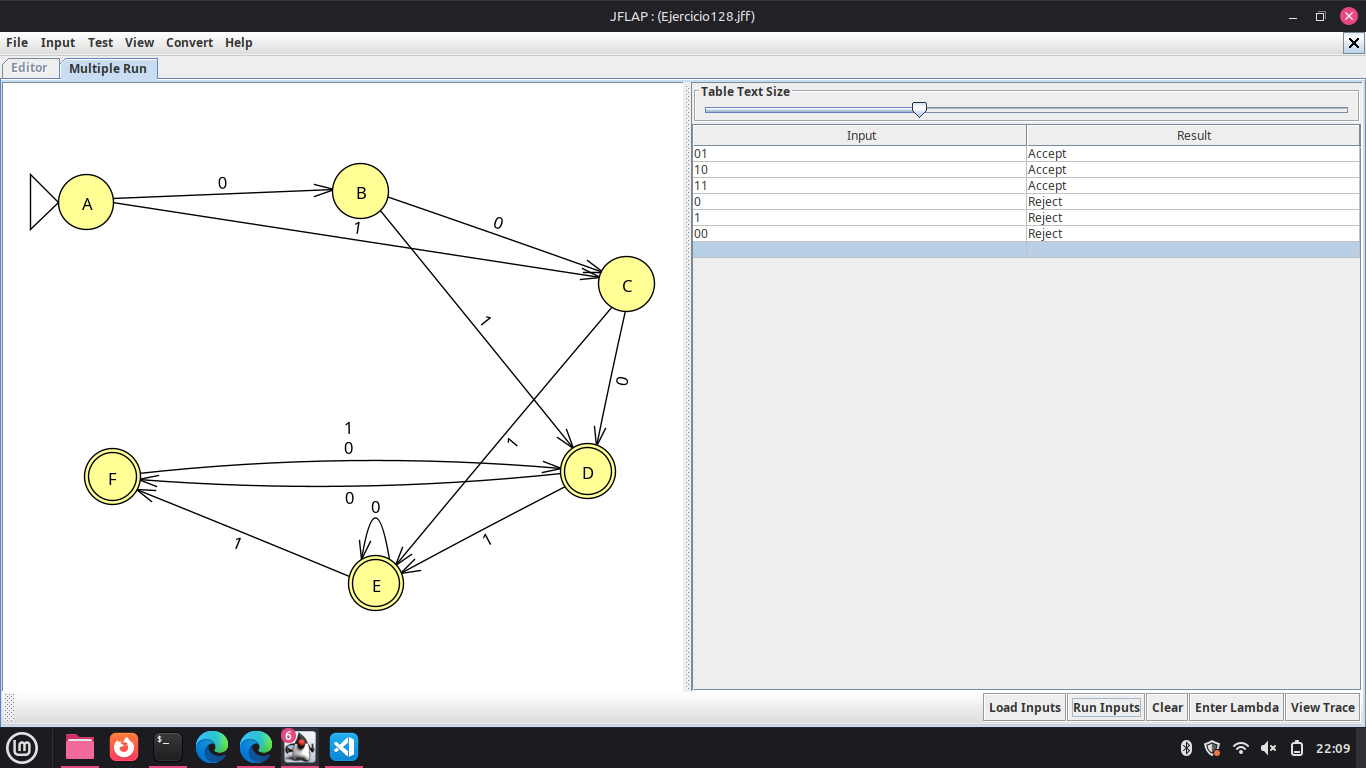
\includegraphics[width=0.95\textwidth]{evidencias/Ejercicio128.png}
\caption{AFD construido para el lenguaje $L_2$ del ejercicio 128.}
\end{figure}

\begin{enunciado}{131}
Dibuje el AFD dado por los siguientes elementos:
\[
M=(\{q_1,q_2\},\{0,1\},\delta,q_1,\{q_2\}).
\]

La función de transición $\delta$ está definida como sigue:
\[
\delta(q_1,0)=q_1
\]
y
\[
\delta(q_2,0)=q_1,
\]
\[
\delta(q_1,1)=q_2
\]
y
\[
\delta(q_2,1)=q_2.
\]

Determine un lenguaje $L(M)$ que el AFD reconoce.
\end{enunciado}
\subsection*{Procedimiento}

El AFD está definido por

\[
M=(\{q_1,q_2\},\{0,1\},\delta,q_1,\{q_2\}).
\]

El estado $q_1$ es inicial y $q_2$ es el único estado de aceptación.

\subsection*{Tabla de transición}

\begin{center}
\begin{tabular}{c|cc}
Estado & 0 & 1 \\ \hline
$\rightarrow q_1$ & $q_1$ & $q_2$ \\
$*q_2$ & $q_1$ & $q_2$
\end{tabular}
\end{center}

Se observa que al leer un $0$ el autómata termina en $q_1$, mientras que
al leer un $1$ termina en $q_2$.

Por lo tanto, el lenguaje reconocido es

\[
\boxed{
L(M)=\{w\in\{0,1\}^*:w\text{ termina en }1\}
}
\]

\subsection*{Evidencia en JFLAP}

\begin{figure}[H]
\centering
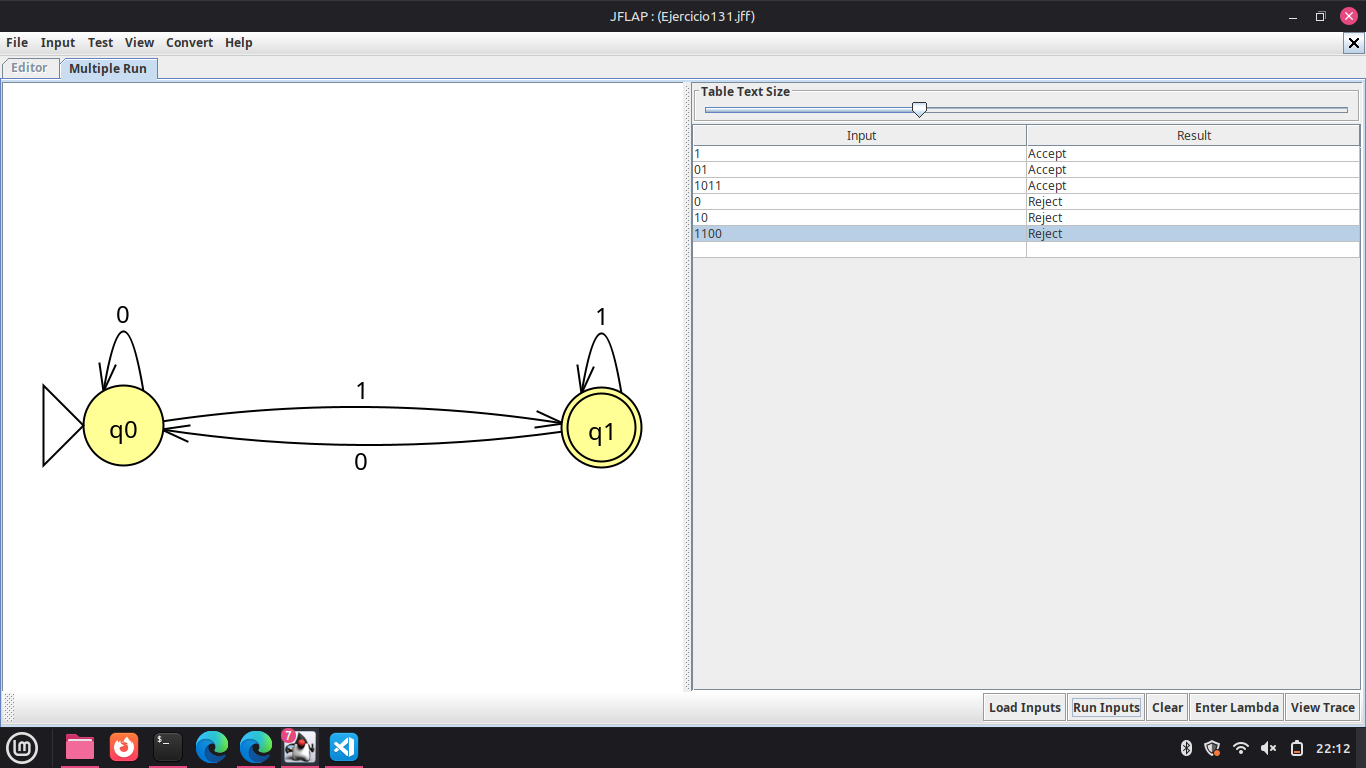
\includegraphics[width=0.95\textwidth]{evidencias/Ejercicio131.png}
\caption{AFD correspondiente al ejercicio 131.}
\end{figure}

\begin{enunciado}{133}
Obtener la tabla de estados y el diagrama de transiciones (esquema AFD)
del autómata finito
\[
M=(Q,\Sigma,\delta,q_0,F),
\]
donde:

\[
Q=\{q_0,q_1,q_2,q_3\},
\]

\[
\Sigma=\{a,b\},
\]

$q_0$ es el estado inicial y también el estado final
$(F=\{q_0\})$.

Las transiciones están definidas de la siguiente manera:
\[
\begin{aligned}
\delta(q_0,a)&=q_2, &
\delta(q_3,a)&=q_1, &
\delta(q_2,b)&=q_3,\\
\delta(q_1,a)&=q_3, &
\delta(q_0,b)&=q_1, &
\delta(q_3,b)&=q_2,\\
\delta(q_2,a)&=q_0, &
\delta(q_1,b)&=q_0.
\end{aligned}
\]
\end{enunciado}


\begin{enunciado}{135}
Dado
\[
\Sigma=\{a,b\},
\]
construir un AFD que reconozca el lenguaje:
\[
L=\{b^mab^n:m,n>0\}.
\]
\end{enunciado}


\begin{enunciado}{137}
Construir un AFD que reconozca el conjunto de todas las cadenas sobre
\[
\Sigma=\{a,b\}
\]
que comiencen con el prefijo ``ab''.
\end{enunciado}


\begin{enunciado}{139}
Determine un autómata finito (FA) que acepte todas las cadenas en
\[
\{0,1\}^*
\]
que tengan un número par de ceros.
\end{enunciado}


\begin{enunciado}{141}
Determine un autómata finito (FA), $M$, que acepte el lenguaje $L$, donde:
\[
L=\{w\in\{0,1\}^*: \text{cada }0\text{ en }w\text{ tiene un }1
\text{ inmediatamente a su derecha}\}.
\]
\end{enunciado}


\begin{enunciado}{143}
Determine los lenguajes producidos por los autómatas finitos (FA)
mostrados en las Figuras (a) y (b).
\end{enunciado}


\begin{enunciado}{145}
Encuentre un AFD que lee un número binario de derecha a izquierda e
identifica aquellos que son múltiplos de 5.
\end{enunciado}


\begin{enunciado}{147}
Diseñe un AFD que lee un número binario de izquierda a derecha y lo
acepta si es un múltiplo de 6.
\end{enunciado}


\begin{enunciado}{148}
Diseñar un autómata finito (FA) que modele el progreso de un alumno de la
ESCOM a lo largo de una Unidad de Aprendizaje, en este caso el curso de
Teoría de la Computación.

El autómata debe representar las distintas decisiones que se toman en cada
evaluación, como si el alumno aprueba, aplaza o no se presenta a un examen,
y controlar que no se presenten más de dos convocatorias en un año.

El autómata concluirá cuando el alumno apruebe el curso.

El alfabeto de entrada estará formado por los siguientes elementos:

\begin{itemize}
    \item $P$: El alumno se presenta al examen.
    \item $N$: El alumno no se presenta al examen.
    \item $A$: El alumno aprueba el examen.
    \item $S$: El alumno aplaza el examen.
\end{itemize}

El alumno comenzará en un estado inicial y tomará decisiones sobre si
presentarse en las distintas convocatorias de febrero, septiembre y
diciembre, hasta que apruebe el curso.

Se deben evitar más de dos convocatorias en un año y reiniciar el ciclo en
caso de no aprobar en las dos primeras.
\end{enunciado}


\begin{enunciado}{149}
Considere el autómata
\[
A=(Q,\Sigma,\delta,A_0,F)
\]
definido en la siguiente tabla.

Encuentre $Q$, $\Sigma$, $A_0$ y $F$, haga el diagrama de transiciones
del autómata y halle los valores que se piden en cada inciso.

\[
\begin{array}{c|cc}
 & 0 & 1\\
\hline
\rightarrow A & B & C\\
B & A & C\\
* C & C & A
\end{array}
\]

\begin{enumerate}[label=\alph*)]
    \item $\delta(B,0)$
    
    \item $\delta(C,1)$
    
    \item $\hat{\delta}(A,1101)$
    
    \item $\hat{\delta}(A,01001)$
\end{enumerate}
\end{enunciado}


\begin{enunciado}{150}
Considere el autómata
\[
A=(Q,\Sigma,\delta,A_0,F)
\]
definido en la siguiente tabla.

Encuentre $Q$, $\Sigma$, $A_0$ y $F$, haga el diagrama de transiciones
del autómata y halle los valores que se piden en cada inciso.

\[
\begin{array}{c|ccc}
 & 0 & 1 & a\\
\hline
\rightarrow A & B & C & D\\
* B & B & C & C\\
* C & A & A & D\\
* D & B & B & B
\end{array}
\]

\begin{enumerate}[label=\alph*)]
    \item $\hat{\delta}(B,10a11)$
    
    \item $\hat{\delta}(B,aa1100)$
    
    \item $\hat{\delta}(A,a01a01)$
    
    \item $\hat{\delta}(C,a11a00)$
\end{enumerate}
\end{enunciado}



\end{document}